\section{Antiderivatives and Indefinite Integration}\label{sec:antider}

We have spent considerable time considering the derivatives of a function and their applications. In the following chapters, we are going to starting thinking in ``the other direction.'' That is, given a function $f(x)$, we are going to consider functions $F(x)$ such that $F'(x) = f(x)$. There are numerous reasons this will prove to be useful: these functions will help us compute areas, volumes, mass, force, pressure, work, and much more.




Given a function $y=f(x)$, a \textit{differential equation} is one that incorporates $y$, $x$, and the derivatives of $y$. For instance, a simple differential equation is: $$y' = 2x.$$

Solving a differential equation amounts to finding a function $y$ that satisfies the given equation. Take a moment and consider that equation; can you find a function $y$ such that $y' = 2x$?

Can you find another?

And yet another?

Hopefully one was able to come up with at least one solution: $y = x^2$. ``Finding another'' may have seemed impossible until one realizes that a function like $y=x^2+1$ also has a derivative of $2x$. Once that discovery is made, finding ``yet another'' is not difficult; the function $y = x^2 + 123,456,789$ also has a derivative of $2x$. The differential equation $y' = 2x$ has many solutions. This leads us to some definitions.
%\enlargethispage{3\baselineskip}

\begin{definition}{Antiderivatives and Indefinite Integrals}{antider}
{Let a function $f(x)$ be given. An \textbf{antiderivative} of $f(x)$ on an open interval $ I $ is a function $F(x)$ such that $\Fp(x) = f(x)$ for all $ x\in I $.\index{antiderivative}\index{indefinite integral}\index{integration!indefinite}\\

The set of all antiderivatives of $f(x)$ is referred to as the \textit{General Antiderivative}, ot the \textbf{(indefinite) integral of $f$}, denoted by $$\int f(x) \ dx.$$
}
\end{definition}

The process of finding the indefinite integral is called \dfont{integration} (or \dfont{integrating $f(x)$}).
Make a note about our definition: we refer to \textit{an} antiderivative of $f$, as opposed to \textit{the} antiderivative of $f$, since there is \textit{always} an infinite number of them. We often use upper-case letters to denote antiderivatives.

Knowing one antiderivative of $f$ allows us to find infinitely more, simply by adding a constant. Not only does this give us \textit{more} antiderivatives, it gives us \textit{all} of them.

\begin{theorem}{Antiderivative Forms}{antideriv_const}
{Let $F(x)$ and $G(x)$ be antiderivatives of $f(x)$. Then there exists a constant $C$ such that $$G(x) = F(x) + C.$$
}
\end{theorem}

To see why this is true, observe that if $ F $ and $ G $ are both antiderivatives of $ f $, then $ F'=G'=f $, so $ \frac{d}{dx}(G-F)=G'-F'=f-f=0$, so $ G-F $ is a constant function giving $ G-F=C $, so $ G=F+C$.

So, given a function $f$ and one of its antiderivatives $F$, we know \textit{all} antiderivatives of $f$ have the form $F(x) + C$ for some constant $C$. Using Definition \ref{def:antider}, we can say that $$\int f(x) \ dx = F(x) + C.$$

Let's analyze this indefinite integral notation.\index{integration!notation}


\begin{figure}
\begin{center}
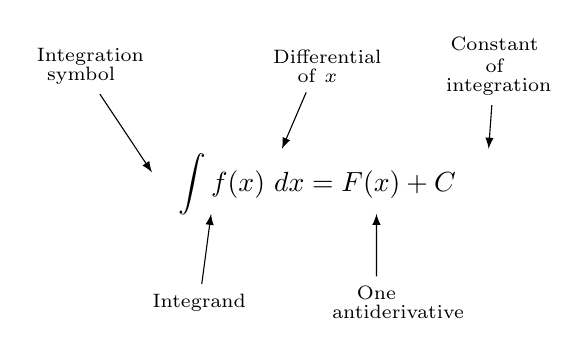
\begin{tikzpicture}[scale=1.5,>=latex]
%\draw [thin,step=1cm] (0,0) grid  (3,3);
\draw  (2,2) node {$\displaystyle \int f(x)\ dx=F(x)+C$};

\draw [{\colorone}] (1,1) node [](a) {\scriptsize Integrand};
\draw [{\colorone},->] (a) -- (1.1,1.75);

\draw [{\colorone}] (0,3) node [text width=32pt,align=center] (b) {\scriptsize \centering Integration\\[-5pt] symbol};
\draw [{\colorone},->] (b) -- (.6,2.1);

\draw [{\colorone}] (2,3) node [text width=32pt,align=center] (c) {\scriptsize \centering Differential\\[-5pt] of $x$};
\draw [{\colorone},->] (c) -- (1.7,2.3);

\draw [{\colorone}] (2.5,1) node [text width=32pt,align=center] (c) {\scriptsize \centering One\\[-5pt] antiderivative};
\draw [{\colorone},->] (c) -- (2.5,1.75);

\draw [{\colorone}] (3.5,3) node [text width=35pt,align=center] (c) {\scriptsize \centering Constant of\\[-5pt] integration};
\draw [{\colorone},->] (c) -- (3.45,2.3);
\end{tikzpicture}

\caption{Understanding the indefinite integral notation.\label{fig:anti1}}
\end{center}
\end{figure}

%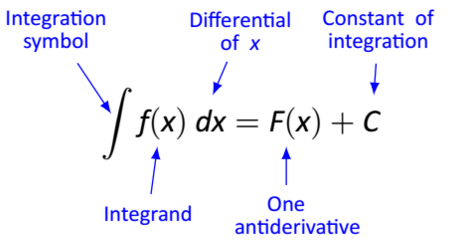
\includegraphics{figures/figanti1}
%\captionsetup{type=figure}%
%\caption{Understanding the indefinite integral notation.}\label{fig:anti1}


Figure \ref{fig:anti1} shows the typical notation of the indefinite integral. The integration symbol, $\int$, is in reality an ``elongated S,'' representing ``take the sum.'' We will later see how \textit{sums} and \textit{antiderivatives} are related.

The function we want to find an antiderivative of is called the \textit{integrand}. It contains the differential of the variable we are integrating with respect to. The $\int$ symbol and the differential $dx$ are not ``bookends'' with a function sandwiched in between; rather, the symbol $\int$ means ``find all antiderivatives of what follows,'' and the function $f(x)$ and $dx$ are multiplied together; the $dx$ does not ``just sit there.''

Let's practice using this notation.\\


\begin{example}{Evaluating indefinite integrals}{ex_anti2}{
Evaluate $\displaystyle \int \sin x\ dx.$}
\end{example}
\begin{solution}
{We are asked to find all functions $F(x)$ such that $\Fp(x) = \sin x$. Some thought will lead us to one solution: $F(x) = -\cos x$, because $\frac{d}{dx}(-\cos x) = \sin x$.

The indefinite integral of $\sin x$ is thus $-\cos x$, plus a constant of integration. So:
$$\int \sin x \ dx = -\cos x + C.$$
\vskip-\baselineskip
} 
\end{solution}


{\bf Common mistakes:}
One habit students make with integrals is to \ifont{drop the dx} at the end of the integral.
This is required! Think of the integral as a set of parenthesis.
Both are required so it is clear where the integrand ends and what variable you are integrating with respect to.

Another common mistake is to \ifont{forget the +C} for indefinite integrals.


A commonly asked question is ``What happened to the $dx$?'' The unenlightened response is ``Don't worry about it. It just goes away.'' A full understanding includes the following.

This process of \textit{antidifferentiation} is really solving a \textit{differential} question. The integral $$\int \sin x\ dx$$ presents us with a differential, $dy = \sin x\ dx$. It is asking: ``What is $y$?'' We found lots of solutions, all of the form $y = -\cos x+C$.

%We can view integration in the following way. 
Letting $dy = \sin x\ dx$,  rewrite 
$$\int \sin x \ dx \quad \text{as}\quad \int  dy.$$
This is asking: ``What functions have a differential of the form $dy$?'' The answer is ``Functions of the form $y+C$, where $C$ is a constant.'' What is $y$? We have lots of choices, all differing by a constant; the simplest choice is $y = -\cos x$.

Understanding all of this is more important later as we try to find antiderivatives of more complicated functions. In this section, we will simply explore the rules of indefinite integration, and one can succeed for now with answering ``What happened to the $dx$?'' with ``It went away.''



Let's practice once more before stating integration rules.\\

\begin{example}{Evaluating indefinite integrals}{ex_anti3}{
Evaluate $\ds \int (3x^2 + 4x+5)\ dx$.}
\end{example}

\begin{solution}
{We seek a function $F(x)$ whose derivative is $3x^2+4x+5$. When taking derivatives, we can consider functions term--by--term, so we can likely do that here.

What functions have a derivative of $3x^2$? Some thought will lead us to a cubic, specifically $x^3+C_1$, where $C_1$ is a constant. 

What functions have a derivative of $4x$? Here the $x$ term is raised to the first power, so we likely seek a quadratic. Some thought should lead us to $2x^2+C_2$, where $C_2$ is a constant.

Finally, what functions have a derivative of $5$? Functions of the form $5x+C_3$, where $C_3$ is a constant.

Our answer appears to be 
$$\int (3x^2+4x+5)\ dx = x^3+C_1+2x^2+C_2+5x+C_3.$$ We do not need three separate constants of integration; combine them as one constant, giving the final answer of 
$$\int (3x^2+4x+5)\ dx = x^3+2x^2+5x+C.$$

It is easy to verify our answer; take the derivative of $x^3+2x^3+5x+C$ and see we indeed get $3x^2+4x+5$.
}
\end{solution}


This final step of ``verifying our answer'' is important both practically and theoretically. In general, taking derivatives is easier than finding antiderivatives so checking our work is easy and vital as we learn.

We also see that taking the derivative of our answer returns the function in the integrand. Thus we can say that: $$\frac{d}{dx}\left(\int f(x)\ dx\right) = f(x).$$
Differentiation ``undoes'' the work done by antidifferentiation. 

The table at the end of Chapter 4  gave a list of the derivatives of common functions we had learned at that point. We restate part of that list here to stress the relationship between derivatives and antiderivatives. This list will also be useful as a glossary of common antiderivatives as we learn.

%\newlength{\bh}%box height
%\newlength{\bd}%box depth
%\settoheight{\bh}{$\frac{d}{dx}$}
%\settodepth{\bd}{$\frac{d}{dx}$}

%\newcommand{\myrule}{\rule[-\bd]{0pt}{\bh+\bd}}%\ $\frac{d}{dx}$
%\newcommand{\myrule}{\rule[-4pt]{0pt}{13pt}}%\ $\frac{d}{dx}$

\begin{theorem}{Derivatives and Antiderivatives}{indef_alg}
\begin{minipage}[t]{.45\textwidth}
Common Differentiation Rules\rule[-2pt]{0pt}{1pt}
\begin{enumerate}
\item \myrule$\frac{d}{dx}\big(cf(x) \big) = c\cdot \fp(x)$
\item \myrule$\frac{d}{dx}\big(f(x)\pm g(x) \big) = $
\vskip .05\baselineskip
\myrule$\fp(x)\pm g'(x)$
\item $\frac{d}{dx}\big(C \big) = 0$\myrule
\item $\frac{d}{dx}\big(x \big) = 1$\myrule
\item $\frac{d}{dx}\big(x^n \big) = n\cdot x^{n-1}$\myrule
\item $\frac{d}{dx}\big(\sin x \big) = \cos x$\myrule
\item $\frac{d}{dx}\big(\cos x \big) = -\sin x$\myrule
\item $\frac{d}{dx}\big(\tan x \big) = \sec^2 x$\myrule
\item $\frac{d}{dx}\big(\csc x \big) = -\csc x\cot x$\myrule
\item $\frac{d}{dx}\big(\sec x \big) = \sec x\tan x$\myrule
\item $\frac{d}{dx}\big(\cot x \big) = -\csc^2 x$\myrule
\item $\frac{d}{dx}\big(e^ x \big) = e^x$\myrule
\item $\frac{d}{dx}\big(a^x \big) = \ln a\cdot a^x$\myrule
\item $\frac{d}{dx}\big(\ln x \big) =\frac{d}{dx}\big(\ln |x| \big) = \frac1 x$\myrule
\item $\frac{d}{dx}\big(\cosh x\big) = \sinh x$
\item $\frac{d}{dx}\big(\sinh x\big) = \cosh x$
\item $\frac{d}{dx}\big(\ln(\cosh x)\big) = \tanh x$
\item $\frac{d}{dx}\big(\ln(\sinh x)\big) = \coth x$
\item $\ds \frac{d}{dx}\big(\sin^{-1}(x)\big) = \frac{1}{\sqrt{1-x^2}}$ \label{invsin} 
%\item $\ds \frac{d}{dx}\big(\sec^{-1}(x)\big) = \frac{1}{ x \sqrt{x^2-1}}$
\item $\ds \frac{d}{dx}\big(\tan^{-1}(x)\big) = \frac{1}{1+x^2}$ \label{invtan}
%\item $\frac{d}{dx}\big(\csch x\big) = -\csch x\coth x$
%\item $\frac{d}{dx}\big(\coth x\big) = -\csch^2x$

\end{enumerate}
\end{minipage}
\begin{minipage}[t]{.55\textwidth}
Common Indefinite Integral Rules\rule[-2pt]{0pt}{1pt}
\begin{enumerate}
\item \myrule$\int c\cdot f(x)\ dx = c\cdot \int f(x)\ dx$
\item \myrule$\int \big(f(x)\pm g(x)\big)\ dx =$
\vskip .05\baselineskip
\myrule$ \int f(x)\ dx\pm \int g(x)\ dx$
\item $\int 0\ dx = C$\myrule
\item $\int 1\ dx = \int dx = x+C$\myrule
\item $\int x^n\ dx =\frac{1}{n+1}x^{n+1}+ C$\quad {\scriptsize ($n\neq -1$)}\myrule
\item $\int \cos x\ dx = \sin x+C$\myrule
\item $\int \sin x\ dx = -\cos x+C$\myrule
\item $\int \sec^2 x\ dx = \tan x+C$\myrule
\item $\int \csc x\cot  x\ dx = -\csc x+C$\myrule
\item $\int \sec x\tan x\ dx = \sec x+C$\myrule
\item $\int \csc^2 x\ dx = -\cot x+C$\myrule
\item $\int e^x\ dx = e^x+C$\myrule
\item $\int a^x\ dx = \frac{1}{\ln a}\cdot a^x+C$\myrule
\item $\int \frac{1}x\ dx = \ln |x|+C$\myrule
\item $\ds\int \cosh x\ dx = \sinh x+C$ \myrule
\item $\ds\int \sinh x\ dx = \cosh x+C$ \myrule
\item $\ds\int \tanh x\ dx = \ln(\cosh x) +C$ \myrule
\item $\ds\int \coth x\ dx = \ln|\sinh x\,|+C$ \myrule
\item $\ds     \int \frac{1}{\sqrt{1-x^2}} dx = \sin^{-1}(x) +C $ 
%\item $\ds \frac{d}{dx}\big(\sec^{-1}(x)\big) = \frac{1}{ x \sqrt{x^2-1}}$
\item $\ds  \int \frac{1}{1+x^2} \; dx = \tan^{-1}(x) +C$
\end{enumerate}
\end{minipage}%\\
%
%\textit{\small (continued $\ldots$)}
\end{theorem}
%\addtocounter{theoremcounter}{-1}
%
%\theorem{thm:indef_algb}{Derivatives and Antiderivatives -- Continued}
%{\begin{minipage}[t]{.45\specialboxlength}
%Common Differentiation Rules\rule[-2pt]{0pt}{1pt}
%\begin{enumerate}\addtocounter{enumi}{5}
%%\item \myrule$\frac{d}{dx}\big(cf(x) \big) = c\cdot \fp(x)$
%%\item \myrule$\frac{d}{dx}\big(f(x)\pm g(x) \big) = $
%%\vskip .05\baselineskip
%%\myrule$\fp(x)\pm g'(x)$
%%\item $\frac{d}{dx}\big(C \big) = 0$\myrule
%%\item $\frac{d}{dx}\big(x \big) = 1$\myrule
%%\item $\frac{d}{dx}\big(x^n \big) = n\cdot x^{n-1}$\myrule
%\item $\frac{d}{dx}\big(\sin x \big) = \cos x$\myrule
%\item $\frac{d}{dx}\big(\cos x \big) = -\sin x$\myrule
%\item $\frac{d}{dx}\big(\tan x \big) = \sec^2 x$\myrule
%\item $\frac{d}{dx}\big(\csc x \big) = -\csc x\cot x$\myrule
%\item $\frac{d}{dx}\big(\sec x \big) = \sec x\tan x$\myrule
%\item $\frac{d}{dx}\big(\cot x \big) = -\csc^2 x$\myrule
%\item $\frac{d}{dx}\big(e^ x \big) = e^x$\myrule
%\item $\frac{d}{dx}\big(a^x \big) = \ln a\cdot a^x$\myrule
%\item $\frac{d}{dx}\big(\ln x \big) = \frac1 x$\myrule
%\end{enumerate}
%\end{minipage}
%\begin{minipage}[t]{.55\specialboxlength}
%Common Indefinite Integral Rules\rule[-2pt]{0pt}{1pt}
%\begin{enumerate}\addtocounter{enumi}{5}
%%\item \myrule$\int c\cdot f(x)\ dx = c\cdot \int f(x)\ dx$
%%\item \myrule$\int \big(f(x)\pm g(x)\big)\ dx =$
%%\vskip .05\baselineskip
%%\myrule$ \int f(x)\ dx\pm \int g(x)\ dx$
%%\item $\int 0\ dx = C$\myrule
%%\item $\int 1\ dx = \int dx = x+C$\myrule
%%\item $\int x^n\ dx =\frac{1}{n+1}x^{n+1}+ C$\quad {\scriptsize ($n\neq -1$)}\myrule
%\item $\int \cos x\ dx = \sin x+C$\myrule
%\item $\int \sin x\ dx = -\cos x+C$\myrule
%\item $\int \sec^2 x\ dx = \tan x+C$\myrule
%\item $\int \csc x\cot  x\ dx = -\csc x+C$\myrule
%\item $\int \sec x\tan x\ dx = \sec x+C$\myrule
%\item $\int \csc^2 x\ dx = -\cot x+C$\myrule
%\item $\int e^x\ dx = e^x+C$\myrule
%\item $\int a^x\ dx = \frac{1}{\ln a}\cdot a^x+C$\myrule
%\item $\int \frac{1}x\ dx = \ln |x|+C$\myrule
%\end{enumerate}
%\end{minipage}
%}


We highlight a few important points from Theorem \ref{thm:indef_alg}:
\begin{itemize}
	\item		Rule \#1 states $\int c\cdot f(x)\ dx = c\cdot \int f(x)\ dx$. This is the Constant Multiple Rule: \index{Constant Multiple Rule!of integration} we can temporarily ignore constants when finding antiderivatives, just as we did when computing derivatives (i.e., $\frac{d}{dx}\big(3x^2\big)$ is just as easy to compute as $\frac{d}{dx}\big(x^2\big)$). An example:
	$$\int 5\cos x\ dx = 5\cdot\int \cos x\ dx = 5\cdot (\sin x+C) = 5\sin x + C.$$
	In the last step we can consider the constant as also being multiplied by 5, but ``5 times a constant'' is still a constant, so we just write ``$C$\,''.
	\item		Rule \#2 is the Sum/Difference Rule:\index{integration!Sum/Difference Rule}\index{Sum/Difference Rule!of integration} we can split integrals apart when the integrand contains terms that are added/subtracted, as we did in Example \ref{ex_anti3}. So:
	\begin{align*}
	\int(3x^2+4x+5)\ dx &= \int 3x^2\ dx + \int 4x\ dx + \int 5\ dx \\
											&= 3\int x^2\ dx + 4\int x\ dx + \int 5 \ dx\\
											&= 3\cdot \frac13x^3 + 4\cdot \frac12x^2+5x+C\\
											&= x^3+2x^2+5x+C
	\end{align*}
	In practice we generally do not write out all these steps, but we demonstrate them here for completeness.
	\item		Rule \#5 is the Power Rule of indefinite integration.\index{integration!Power Rule}\index{Power Rule!integration} There are two important things to keep in mind:
		\begin{enumerate}
		\item		Notice the restriction that $n\neq -1$. This is important: $\int \frac{1}{x}\ dx \neq $ ``$\frac{1}{0}x^0+C$''; rather, see Rule \#14.
		\item		We are presenting antidifferentiation as the ``inverse operation'' of differentiation. Here is a useful quote to remember:
		\begin{quote}%\centering
		``Inverse operations do the opposite things in the opposite order.''
		\end{quote}
		When taking a derivative using the Power Rule, we \textbf{first} \textit{multiply} by the power, then \textbf{second} \textit{subtract} 1 from the power. To find the antiderivative, do the opposite things in the opposite order: \textbf{first} \textit{add} one to the power, then \textbf{second} \textit{divide} by the power.
			\end{enumerate}
		\item		Note that Rule \#14 incorporates the absolute value of $x$. The exercises will work the reader through why this is the case; for now, know the absolute value is important and cannot be ignored.
\end{itemize}


Note that we don't have properties to deal with products or quotients of functions, that is, in general
%Just like with derivatives, the following will \dfont{NOT} work:
$$\int f(x)\cdot g(x)\,dx\neq \int f(x)\,dx\int g(x)\,dx.$$
$$\int \frac{f(x)}{g(x)}\,dx\neq \frac{\int f(x)\,dx}{\int g(x)\,dx}.$$
With derivatives, we had the product and quotient rules to deal with these cases.
For integrals, we have no such rules, but we will learn a variety of different techniques to deal with these cases.


\begin{example}{Indefinite Integral}{IndefiniteIntegral2}
If $f'(x)=x^4+2x-8\sin x$ then what is $f(x)$?
\end{example}

\begin{solution} 
The answer is:
$$\begin{array}{rcl}
\ds{f(x)=\int f'(x)\,dx}&=&\ds{\int \left(x^4+2x-8\sin x\right)\,dx}\\
\\
&=&\ds{ \int x^4 \,dx + 2\int x\,dx -8 \int \sin x\,dx }\\
\\
&=&\ds{\frac{x^5}{5}+x^2+8\cos x+C,}\\
\end{array}$$
where $C$ is a constant.
\end{solution}

\begin{example}{Indefinite Integral}{IndefiniteIntegral3}
Find the indefinite integral: $\ds\int 3x^2\,dx$.
\end{example}
\begin{solution}
	$$\begin{array}{rcl}
	\ds{\int 3x^2\,dx} & = & \ds{3\int x^2\,dx}\\
	\\
	&=&\ds{3\frac{x^3}{3}+C}\\
	\\
	&=&x^3+C\\
	\end{array} $$
\end{solution}

\begin{example}{Indefinite Integral}{IndefiniteIntegral4}
Find the general antiderivative of $\ds \frac{2}{\sqrt x}\,dx$.
\end{example}
\begin{solution}
	$$\begin{array}{rcl}
	\ds{\int \frac{2}{\sqrt x}\,dx} & = & \ds{2\int x^{-\frac{1}{2}}\,dx}\\
	\\
	&=&\ds{2\frac{x^{-\frac{1}{2}+1}}{-\frac{1}{2}+1}+C}\\
	\\
	&=&4\sqrt x+C\\
	\end{array}$$
\end{solution}

\begin{example}{Indefinite Integral}{IndefiniteIntegral5}
Find:  $\ds\int \left(\frac{1}{x}+e^{7x}+x^\pi+7\right)\,dx$.
\end{example}
\begin{solution}
	$$\begin{array}{rcl}
	\ds{\int \left(\frac{1}{x}+e^{7x}+x^\pi+7\right)\,dx} & = & \ds{\int \frac{1}{x}\,dx+\int e^{7x}\,dx+\int x^\pi\,dx+\int 7\,dx}\\
	\\
	&=& \ds{\ln|x|+\frac{1}{7}e^{7x}+\frac{x^{\pi+1}}{\pi+1}+7x+C}\\
	\end{array}$$
\end{solution}

\subsection*{Differential Equations and Initial Value Problems}
An equation involving derivatives where we want to solve for the original function is called a \dfont{differential equation}.
For example, $f'(x)=2x$ is a differential equation with general solution $f(x)=x^2+C$.
Some solutions (i.e., particular values of $C$) are shown below.
$$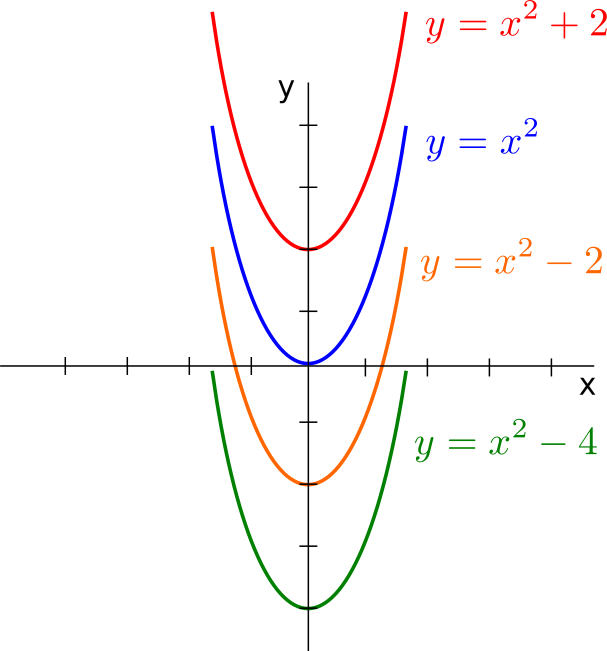
\includegraphics[width=3in]{images2/integral-curves}$$
As seen with integral curves, we may have an infinite family of solutions satisfying the differential equation.
However, if we were given a point (called an \ifont{initial value}) on the curve then we could determine $f(x)$ completely.
Such a problem is known as an \ifont{initial value problem}.

\begin{example}{Initial Value Problem}{Initial Value Problem}
If $f'(x)=2x$ and $f(0)=2$ then determine $f(x)$.
\end{example}

\begin{solution} 
As previously stated, we have a solution of:
$$f(x)=x^2+C.$$
But $f(0)=2$ implies:
$$2=0^2+C\quad\to\quad C=2.$$
Therefore, $f(x)=x^2+2$ is the solution to the initial value problem.
\end{solution}


We have seen that the derivative of a position function is a velocity function, and the derivative of a velocity function describes  acceleration.\index{initial value problem} We can now go ``the other way:'' the antiderivative of an acceleration function gives a velocity function, etc. While there is just one derivative of a given function, there are infinite antiderivatives. Therefore we cannot ask ``What is \textit{the} velocity of an object whose acceleration is $-32$ft/s$^2$?'', since there is more than one answer. 

As above, we can find \textit{the} answer if we provide more information with the question, in the form of an  initial value, a value of the function that one knows beforehand.\\

\begin{example}{Solving initial value problems}{ex_anti4}
The acceleration due to gravity of a falling object is $-32$ ft/s$^2$. At time $t=3$, a falling object had a velocity of $-10$ ft/s. Find the equation of the object's velocity.
\end{example}

\begin{solution}
{We want to know a velocity function, $v(t)$. We know two things:
	\begin{itemize}
		\item		The acceleration, i.e., $v\primeskip'(t)= -32$, and
		\item		the velocity at a specific time, i.e., $v(3) = -10$.
	\end{itemize}
Using the first piece of information, we know that $v(t)$ is an antiderivative of $v\primeskip'(t)=-32$. So we begin by finding the indefinite integral of $-32$:
		$$\int (-32)\ dt = -32t+C=v(t).$$
Now we use the fact that $v(3)=-10$ to find $C$:
\begin{align*}
	v(t) &= -32t+C \\
	v(3) &= -10 \\
	-32(3)+C &= -10\\
	C &= 86
\end{align*}

Thus $v(t)= -32t+86$. We can use this equation to understand the motion of the object: when $t=0$, the object had a velocity of $v(0) = 86$ ft/s. Since the velocity is positive, the object was moving upward.

When did the object begin moving down? Immediately after $v(t) = 0$:
$$-32t+86 = 0 \quad \Rightarrow\quad  t = \frac{43}{16}  \approx 2.69\text{s}.$$
Recognize that we are able to determine quite a bit about the path of the object knowing just its acceleration and its velocity at a single point in time.
}
\end{solution}

\begin{example}{Solving initial value problems}{ex_anti5}
 {
Find $f(t)$, given that $\fpp(t) = \cos t$, $\fp(0) = 3$ and $f(0) = 5$.}
\end{example}

\begin{solution}
{We start by finding $\fp(t)$, which is an antiderivative of $\fpp(t)$:
		$$\int \fpp(t)\ dt = \int \cos t\ dt = \sin t + C = \fp(t).$$
		
		So $\fp(t) = \sin t+C$ for the correct value of $C$. We are given that $\fp(0) = 3$, so:
		$$\fp(0) = 3 \quad \Rightarrow \quad \sin 0+C = 3 \quad \Rightarrow \quad C=3.$$
		Using the initial value, we have found $\fp(t) = \sin t+ 3.$
		
We now find $f(t)$ by integrating again.

%\enlargethispage{3\baselineskip}
$$f(t)=\int \fp(t) \ dt = \int (\sin t+3)\ dt = -\cos t + 3t + C.$$ 
We are given that $f(0) = 5$, so
\begin{align*}
-\cos 0 + 3(0) + C &= 5 \\
-1 + C &= 5\\
C &= 6
\end{align*}
 Thus $f(t) = -\cos t + 3t + 6$.
}
\end{solution}


This section introduced antiderivatives and the indefinite integral. We found they are needed when finding a function given information about its derivative(s). For instance, we found a position function given a velocity function.

In the next section, we will see how position and velocity are unexpectedly related by the areas of certain regions on a graph of the velocity function. Then, in Section \ref{sec:FTC}, we will see how areas and antiderivatives are closely tied together.
